\graphicspath{{Chapters/CrossSection/Figures/}}
\chapter{Observed Events and Cross Section Measurement}
\label{chap:CrossSection}

\section{Observed Events}

The observed and expected event yields after applying the \ZZ\ and \ZZs\ selections are shown
in~\tab{obs-expected-events-seven} for the 7~\tev\ analysis and
in~\tab{obs-expected-events-eight} for the 8~\tev\ analysis. 
A total
of~\ZZSevenTeVNObsZZLLLL\ events
are observed in \LumiPassGRLTwentyEleven~\ifb\ of 7~\tev\ data for the \ZZ\ selection, and a total of~\ZZSevenTeVNObsZZLLLL\ events for the \ZZs\ selection. In the 8~\tev\ data, which corresponds to an integrated luminosity of
\LumiPassGRLTwentyTwelve~\ifb, \ZZEightTeVNObsZZLLLL\ events are observed for
the \ZZ\ selection and \ZZEightTeVNObsZZsLLLL\ for the \ZZs\ selection.

%% Expected and observed events, 7 TeV
\begin{table}
\centering
\small
  \begin{tabular}{lcccc}
    \hline\hline
     7~\tev, \ZZ             & \eeee & \mmmm & \eemm & \llll \\
     \hline
Observed & 16 & 23 & 27 & 66 \\
Exp. Signal &   10.3 $\pm$ 0.1 $\pm$ 1.0 &  16.5 $\pm$ 0.2 $\pm$ 0.9 &  26.7 $\pm$ 0.2 $\pm$ 1.7 &  53.4 $\pm$ 0.3 $\pm$ 3.2 \\
Exp. Bg. & 0.5 $\pm$ 0.6 $\pm$ 0.3 & $<0.6$ & 0.7 $\pm$ 0.7 $\pm$ 0.6 & 0.9 $\pm$ 1.1 $\pm$ 0.7 \\
\hline\hline
    \\
    \hline\hline
     7~\tev, \ZZs             & \eeee & \mmmm & \eemm & \llll \\
     \hline
Observed & 21 & 30 & 33 & 84 \\
Exp. Signal &  12.3 $\pm$ 0.2 $\pm$ 1.2 &  20.5 $\pm$ 0.2 $\pm$ 1.1 &  31.6 $\pm$ 0.3 $\pm$ 2.0 &  64.4 $\pm$ 0.4 $\pm$ 4.0 \\
Exp. Bg. & 4.3 $\pm$ 1.4 $\pm$ 0.6 & $<0.9$ & 5.8 $\pm$ 1.6 $\pm$ 0.9 & 9.1 $\pm$ 2.3 $\pm$ 1.3 \\
    \hline\hline
  \end{tabular}

      \caption[Expected and observed events in \LumiPassGRLTwentyEleven~\ifb\ of
      7~\tev\ data.]
      {Number of observed events passing the \ZZllll\ (top table) and \ZZsllll\
      (bottom table) selections in \LumiPassGRLTwentyEleven~\ifb\ of 7~\tev\
      data, as well as the expected number of signal events (Exp. Signal) and
      the expected background (Exp. Bg.) from the data-driven background
      estimate.  The first uncertainty is statistical, while the second is
      systematic; uncertainties on the integrated luminosity
      (\LumiUncTwentyEleven) are not included.  }
\label{table:obs-expected-events-seven}
\end{table}

%% Expected and observed events, 8 TeV
\begin{table}
\centering
\small
  \begin{tabular}{lcccc}
    \hline\hline
     8~\tev, \ZZ             & \eeee & \mmmm & \eemm & \llll \\
     \hline
Observed & \ZZEightTeVNObsZZEEEE & \ZZEightTeVNObsZZMMMM & \ZZEightTeVNObsZZEEMM & \ZZEightTeVNObsZZLLLL \\
Exp. Signal &   
    \ZZEightTeVNExpZZEEEE~\errSym{\ZZEightTeVNExpStatZZEEEE}~\errSym{\ZZEightTeVNExpStatZZEEEE} & 
    \ZZEightTeVNExpZZMMMM~\errSym{\ZZEightTeVNExpStatZZMMMM}~\errSym{\ZZEightTeVNExpStatZZMMMM} & 
    \ZZEightTeVNExpZZEEMM~\errSym{\ZZEightTeVNExpStatZZEEMM}~\errSym{\ZZEightTeVNExpStatZZEEMM} & 
    \ZZEightTeVNExpZZLLLL~\errSym{\ZZEightTeVNExpStatZZLLLL}~\errSym{\ZZEightTeVNExpStatZZLLLL} \\
Exp. Bg. & 
    \ZZEightTeVNBgZZEEEE~\errSym{\ZZEightTeVNBgStatZZEEEE}~\errSym{\ZZEightTeVNBgStatZZEEEE} & 
    \ZZEightTeVNBgZZMMMM~\errSym{\ZZEightTeVNBgStatZZMMMM}~\errSym{\ZZEightTeVNBgStatZZMMMM} & 
    \ZZEightTeVNBgZZEEMM~\errSym{\ZZEightTeVNBgStatZZEEMM}~\errSym{\ZZEightTeVNBgStatZZEEMM} & 
    \ZZEightTeVNBgZZLLLL~\errSym{\ZZEightTeVNBgStatZZLLLL}~\errSym{\ZZEightTeVNBgStatZZLLLL} \\
\hline\hline
    \\
    \hline\hline
     8~\tev, \ZZs             & \eeee & \mmmm & \eemm & \llll \\
     \hline
Observed & \ZZEightTeVNObsZZEEEE & \ZZEightTeVNObsZZMMMM & \ZZEightTeVNObsZZEEMM & \ZZEightTeVNObsZZLLLL \\
Exp. Signal &   
    \ZZEightTeVNExpZZsEEEE~\errSym{\ZZEightTeVNExpStatZZsEEEE}~\errSym{\ZZEightTeVNExpStatZZsEEEE} & 
    \ZZEightTeVNExpZZsMMMM~\errSym{\ZZEightTeVNExpStatZZsMMMM}~\errSym{\ZZEightTeVNExpStatZZsMMMM} & 
    \ZZEightTeVNExpZZsEEMM~\errSym{\ZZEightTeVNExpStatZZsEEMM}~\errSym{\ZZEightTeVNExpStatZZsEEMM} & 
    \ZZEightTeVNExpZZsLLLL~\errSym{\ZZEightTeVNExpStatZZsLLLL}~\errSym{\ZZEightTeVNExpStatZZsLLLL} \\
Exp. Bg. & 
    \ZZEightTeVNBgZZsEEEE~\errSym{\ZZEightTeVNBgStatZZsEEEE}~\errSym{\ZZEightTeVNBgStatZZsEEEE} & 
    \ZZEightTeVNBgZZsMMMM~\errSym{\ZZEightTeVNBgStatZZsMMMM}~\errSym{\ZZEightTeVNBgStatZZsMMMM} & 
    \ZZEightTeVNBgZZsEEMM~\errSym{\ZZEightTeVNBgStatZZsEEMM}~\errSym{\ZZEightTeVNBgStatZZsEEMM} & 
    \ZZEightTeVNBgZZsLLLL~\errSym{\ZZEightTeVNBgStatZZsLLLL}~\errSym{\ZZEightTeVNBgStatZZsLLLL} \\
    \hline\hline
  \end{tabular}

      \caption[Expected and observed events in \LumiPassGRLTwentyTwelve~\ifb\ of
      8~\tev\ data.]
      {Number of observed events passing the \ZZllll\ (top table) and \ZZsllll\
      (bottom table) selections in \LumiPassGRLTwentyTwelve~\ifb\ of 8~\tev\
      data, as well as the expected number of signal events (Exp. Signal) and
      the expected background (Exp. Bg.) from the data-driven background
      estimate.  The first uncertainty is statistical, while the second is
      systematic; uncertainties on the integrated luminosity
      (\LumiUncTwentyTwelve) are not included.  }
    \label{table:obs-expected-events-eight}
\end{table}

\section{Kinematic Distributions}

\figs{zzdists-Zmass2D-seven}{zzdists-Zmass2D-eight} show the mass of the
subleading \leppair\ versus the mass of the leading \leppair\ for the 7~\tev\
and the 8~\tev\ analyses respectively. In both cases the solid red box
represents the region defined by the mass requirements of the \ZZ\ selection and
the dashed blue box the region defined by those of the \ZZs\ selection. The
events are seen to cluster in the regions where both masses are near \mZ, in
agreement with the \mc\ prediction for the signal (shown as pink boxes, with the
size of the box proportional to the number of expected events).

\fig{zzdists-dr-ptz-seven} shows the correlation between the transverse
momentum of the \leppair s and the opening-angle between the leptons
forming the pair. It is observed that for higher transverse momentum dilepton
pairs the opening-angle tends to be smaller, in good agreement with the \mc\
predictions. 

\figs{zzdists-Zmass-seven}{zzdists-Zmass-eight} show the \dilep\ invariant mass
distributions for the leading and subleading \leppair\ for the 7~\tev\ and
8~\tev\ analyses. ~\fig{zzdists-ZZ-seven} shows the
transverse momentum $\pT^{\ZZ}$ and invariant mass $m^{\ZZ}$ of the four-lepton
system, the transverse momentum of the leading \dilep\ pair $\pt^{Z1}$, and the
transverse momentum of the subleading \dilep\ pair $\pt^{Z2}$, for events
passing the \ZZ\ selection for the 7~\tev\ analysis; \fig{zzdists-ZZ-eight}
shows equivalent figure for the 8~\tev\ analysis.
\figs{zzdists-ZZ-seven}{zzdists-ZZ-eight} show the corresponding
distributions for the \ZZs\ selection for the 7~\tev\ and 8~\tev\ analyses
respectively. In each case the prediction from \mc\ for
the \ZZ\ signal is shown as a pink histogram and the prediction for the
background, taken from \mc\ normalised to the data-driven background estimate,
is shown as a light blue histogram. The shapes of the distributions observed in
data are consistent with these predictions.

%~\fig{zzdists-mindr-mzz-seven} shows the minimum 

% 2D plot, 7 TeV
% Use PDF figure as text alignment is off in eps
 \begin{figure}[htbp]
 \begin{center}
  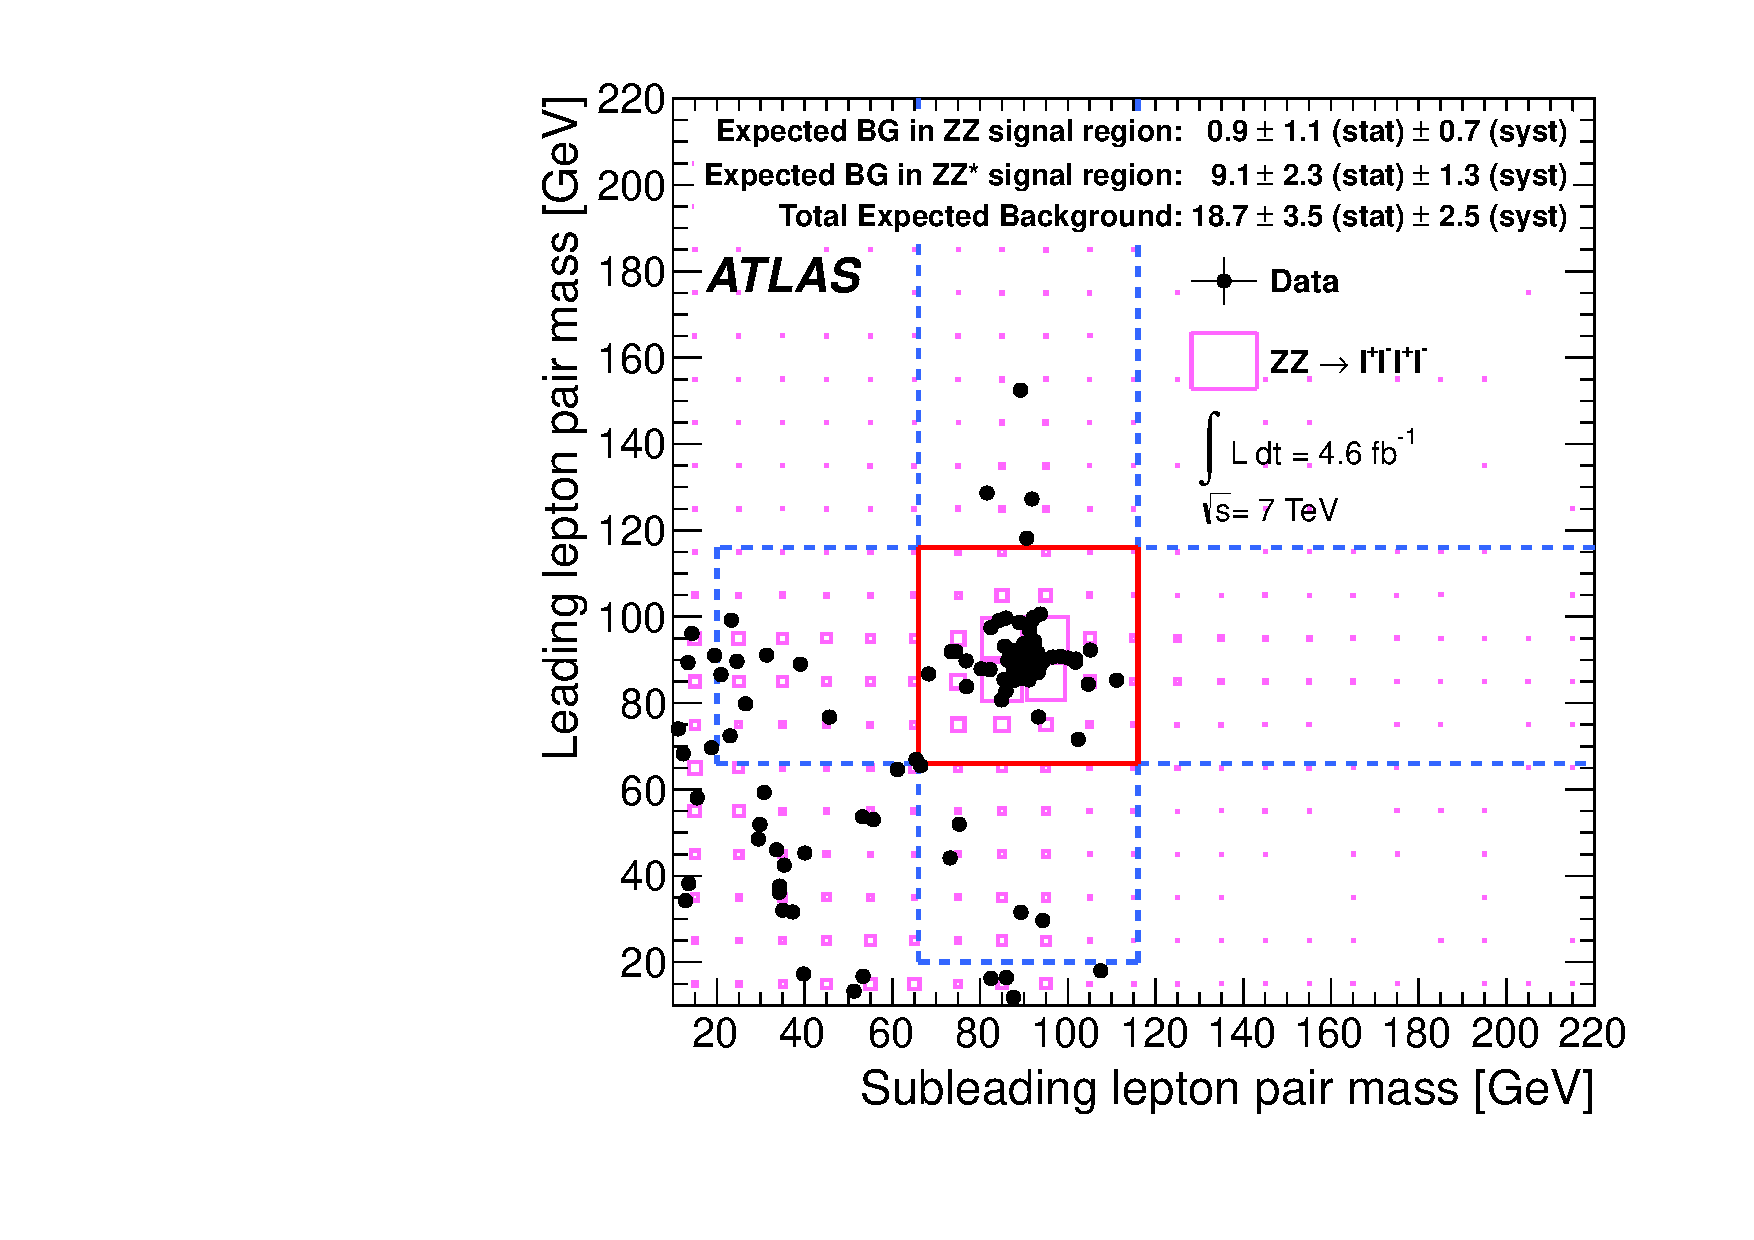
\includegraphics[width=0.7\textwidth]{7TeV/h_mz1_mz2.pdf}\hfill
  \caption[Mass of the leading \leppair\ versus the mass of the
  sub-leading \leppair\ for candidate events in 7~\tev\ data, after applying all of the selection
  requirements apart from the \dilepton\ mass requirements .]
  {\small Mass of the leading \leppair\ versus the mass of the
  sub-leading \leppair\ for candidate events in 7~\tev\ data after
  applying all of the selection
  requirements apart from the \dilepton\ mass requirements.
  The events observed in the data are shown as solid circles and the \ZZsllll\
  signal prediction from simulation as boxes,
  with the size of each box is proportional to the number of events in each bin.  
  The region enclosed by the solid (dashed) lines indicates the signal region defined by the
  \dilepton\ mass requirements for \ZZ\ (\ZZs) events.
  %The background estimate is described in section 5.1.
   }
    \label{fig:zzdists-Zmass2D-seven}
 \end{center}
 \end{figure}

% 2D plot, 8 TeV
% Use PDF figure as text alignment is off in eps
 \begin{figure}[htbp]
 \begin{center}
  
\includegraphics[width=0.7\textwidth]{placeholder}\hfill
  %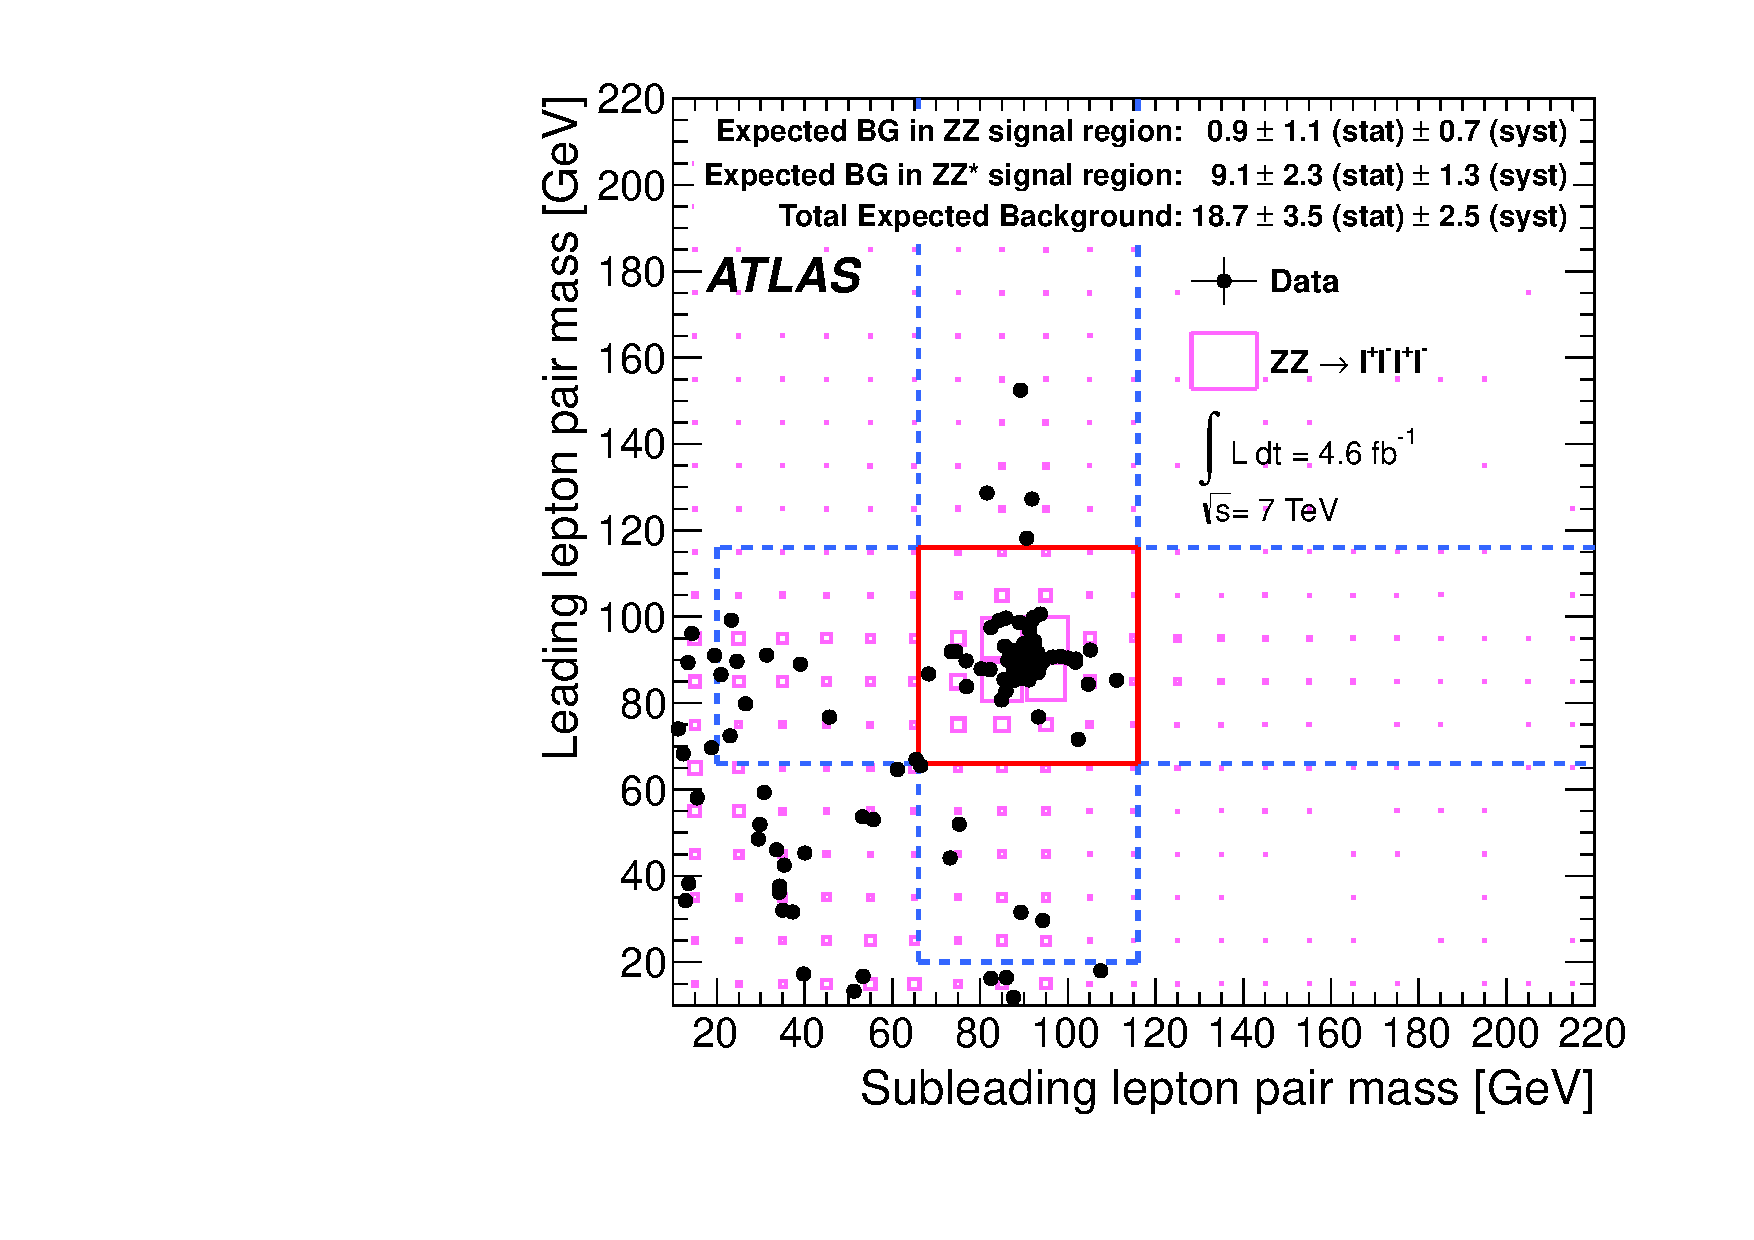
\includegraphics[width=0.7\textwidth]{7TeV/h_mz1_mz2.pdf}\hfill
  \caption[Mass of the leading \leppair\ versus the mass of the
  sub-leading \leppair\ for candidate events in 8~\tev\ data, after applying all of the selection
  requirements apart from the \dilepton\ mass requirements.]
  {\small Mass of the leading \leppair\ versus the mass of the
  sub-leading \leppair for candidate events in 8~\tev\ data after
  applying all of the selection
  requirements apart from the \dilepton\ mass requirements.
  The events observed in the data are shown as solid circles and the \ZZsllll\
  signal prediction from simulation as boxes, with 
  the size of each box is proportional to the number of events in each bin.  
  The region enclosed by the solid (dashed) lines indicates the signal region defined by the
  \dilepton\ mass requirements for \ZZ\ (\ZZs) events.
  %The background estimate is described in section 5.1.
   }
    \label{fig:zzdists-Zmass2D-eight}
 \end{center}
 \end{figure}

% pT_Z vs dR 7 TeV
 \begin{figure}[htbp]
 \begin{center}
  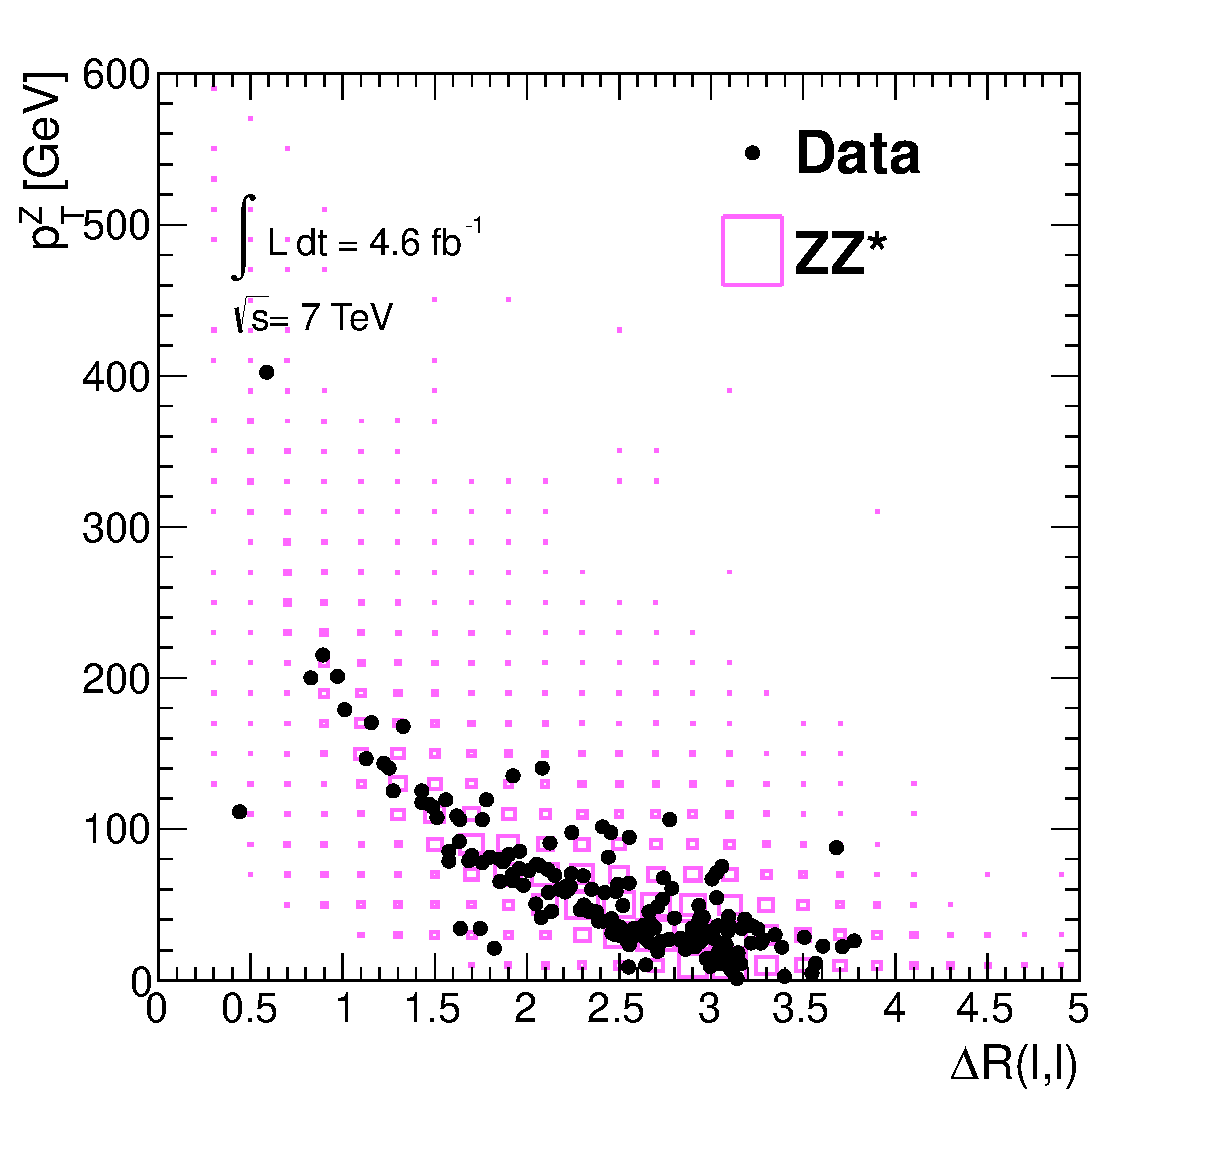
\includegraphics[width=0.7\textwidth]{7TeV/h_dr_ptz}\hfill
  \caption[Transverse momentum of \leppair s versus the opening angle between the two leptons
    forming the pair for events passing the \ZZs\ selection in 7~\tev\ data.]
    {\small Transverse momentum of  \leppair s versus the opening angle between the two leptons
    forming the pair for events passing the \ZZs\ selection in 7~\tev\ data (two
    entries per event).}
 \label{fig:zzdists-dr-ptz-seven}
 \end{center}
 \end{figure}

% m_ZZ vs min(dR) 7 TeV
% !! Not sure what this plot tells us - not much I suspect.
% \begin{figure}[htbp]
% \begin{center}
%  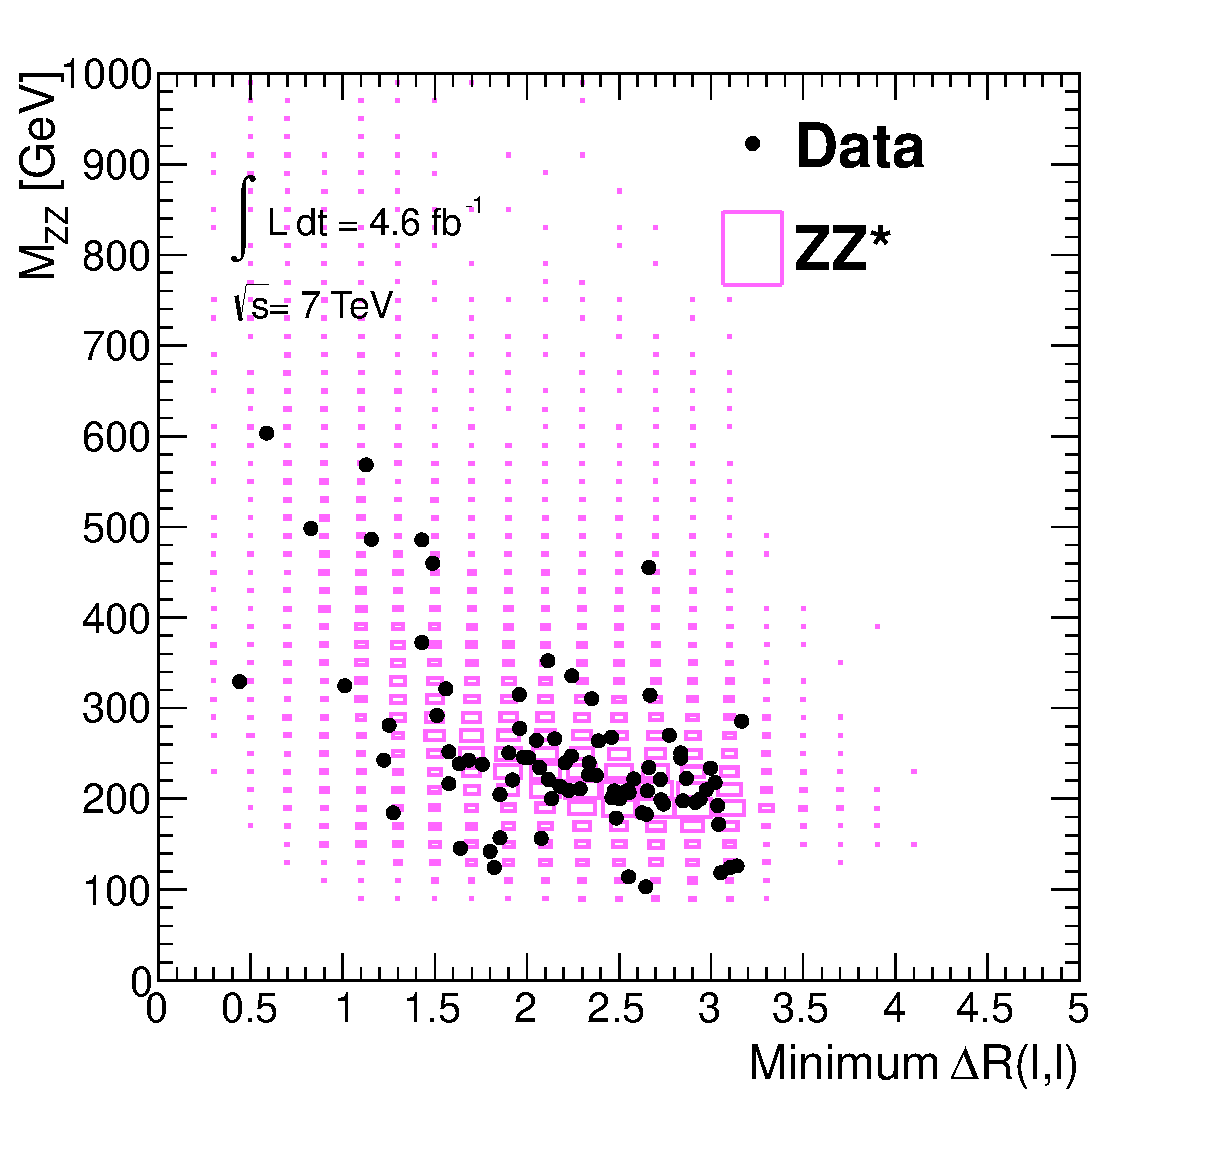
\includegraphics[width=0.7\textwidth]{7TeV/h_mindr_mzz}\hfill
%  \caption[The invariant mass of the four lepton system \mZZp\ versus the
%    minimum \deltaR\ between any pair of leptons in the event for events passing
%    the \ZZs\ selection in 7~\tev\ data.]
%    {\small The invariant mass of the four lepton system \mZZp\ versus the
%    minimum \deltaR\ between any pair of leptons in the event for events passing
%    the \ZZs\ selection in 7~\tev\ data.
%    The events observed in the data are shown as black dots and the signal prediction as boxes.}
% \label{fig:zzdists-mindr-mzz-seven}
% \end{center}
% \end{figure}

% 7 TeV, Z1_m, Z2_m, m_Z>7GeV
\begin{figure}[htbp]
    \begin{center}
     \subfigure[]{
     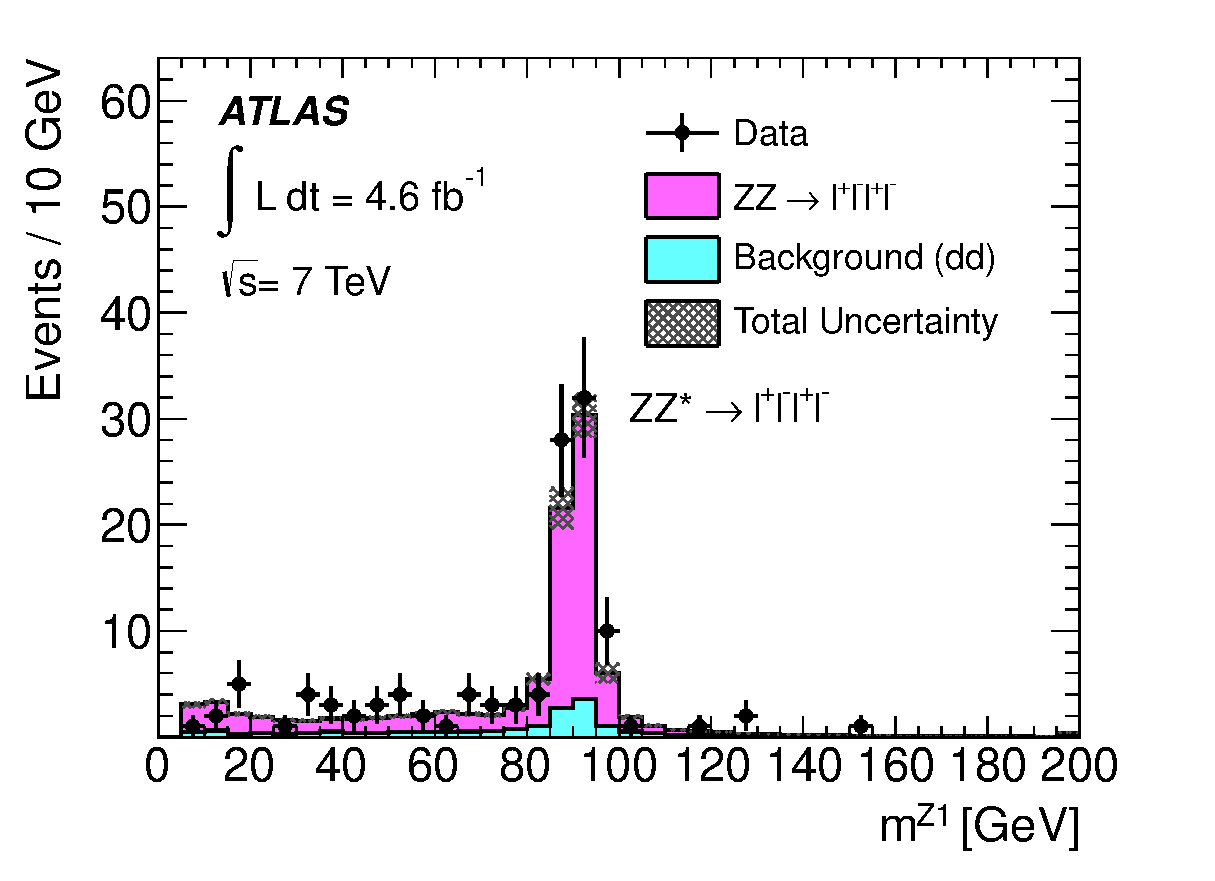
\includegraphics[width=0.47\textwidth]{7TeV/h_4l_ZZs_Z1_m}
     }
     \subfigure[]{
     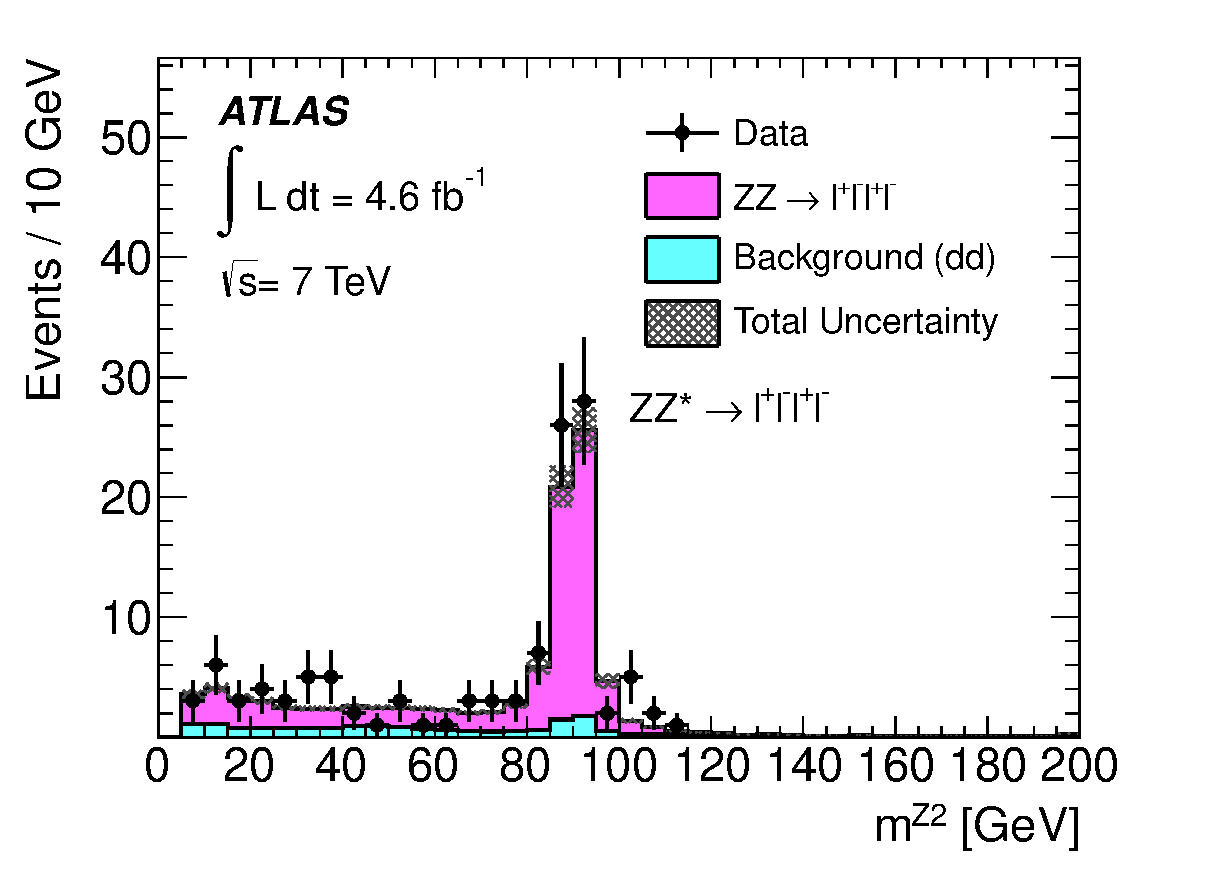
\includegraphics[width=0.47\textwidth]{7TeV/h_4l_ZZs_Z2_m}
     }
    \caption[Invariant masses of the (a) leading and (b) subleading \leppair\
    in candidate \ZZ\ events in the 7~\tev\ data.]
    {Invariant masses of the (a) leading and (b) subleading \leppair\
    in candidate \ZZ\ events in the 7~\tev\ data. Both \leppair s are required to have
    $m_{\ell\ell}>7$~\gev.  The points represent the observed data and the
    histograms show the prediction from simulation, where the background is
    normalized to the data-driven estimate as described in~\chap{BackgroundEstimate}. 
    The shaded band shows the combined statistical and
    systematic uncertainty on the prediction. 
}
    \label{fig:zzdists-Zmass-seven}
\end{center}
\end{figure}

% 7 TeV, ZZ, ZZ_pt / ZZ_m
\begin{figure}[htbp]
    \begin{center}
     \subfigure[]{
     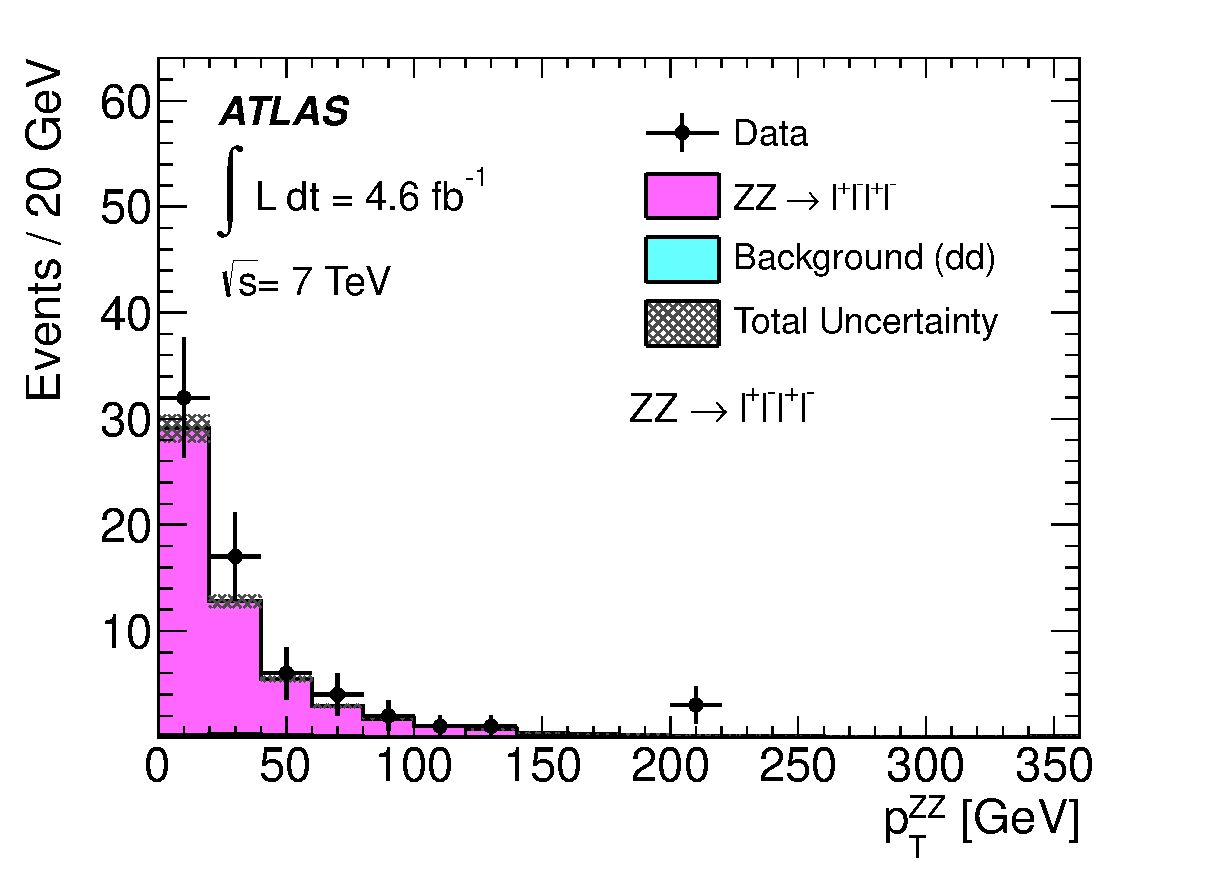
\includegraphics[width=0.47\textwidth]{7TeV/h_4l_ZZ_ZZ_pt}
     }
     \subfigure[]{
     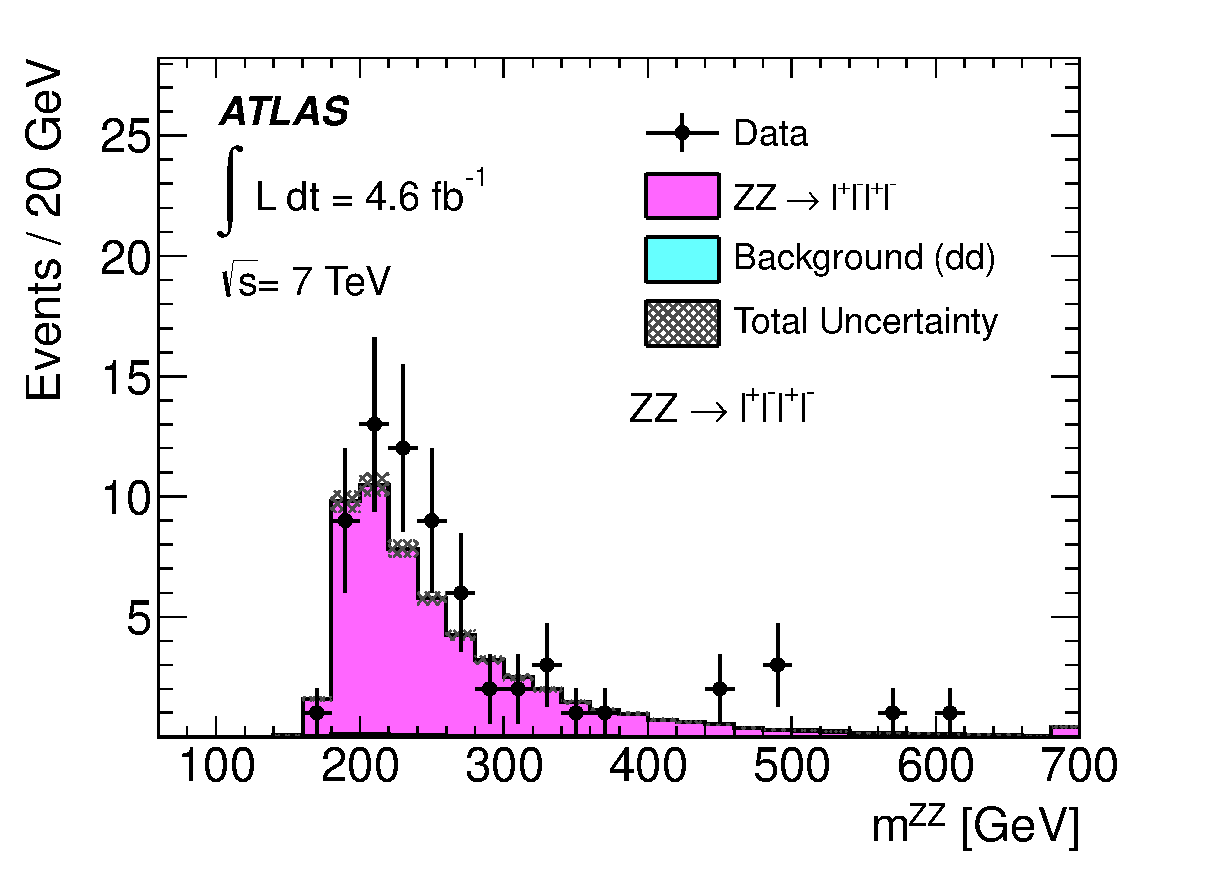
\includegraphics[width=0.47\textwidth]{7TeV/h_4l_ZZ_ZZ_m}
     }
     \subfigure[]{
     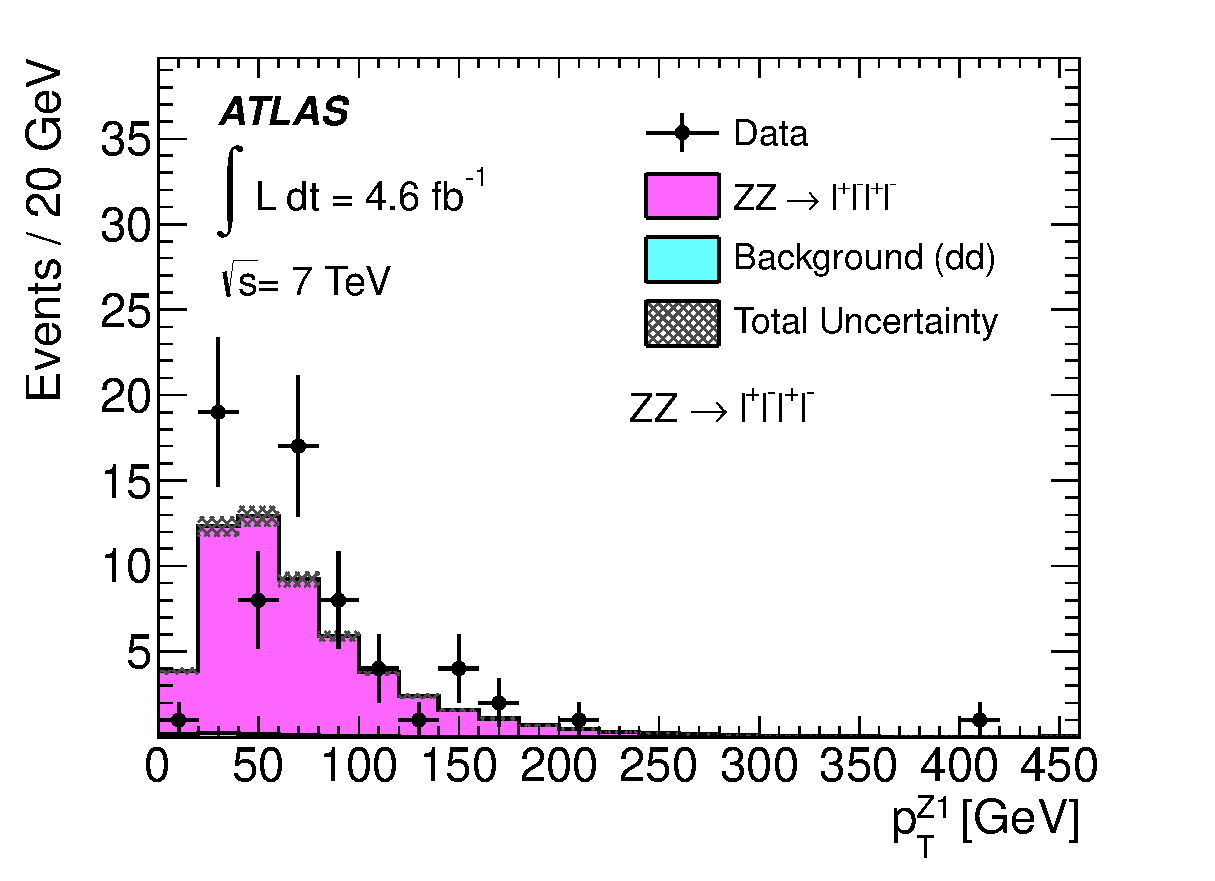
\includegraphics[width=0.47\textwidth]{7TeV/h_4l_ZZ_Z1_pt}
     }
     \subfigure[]{
     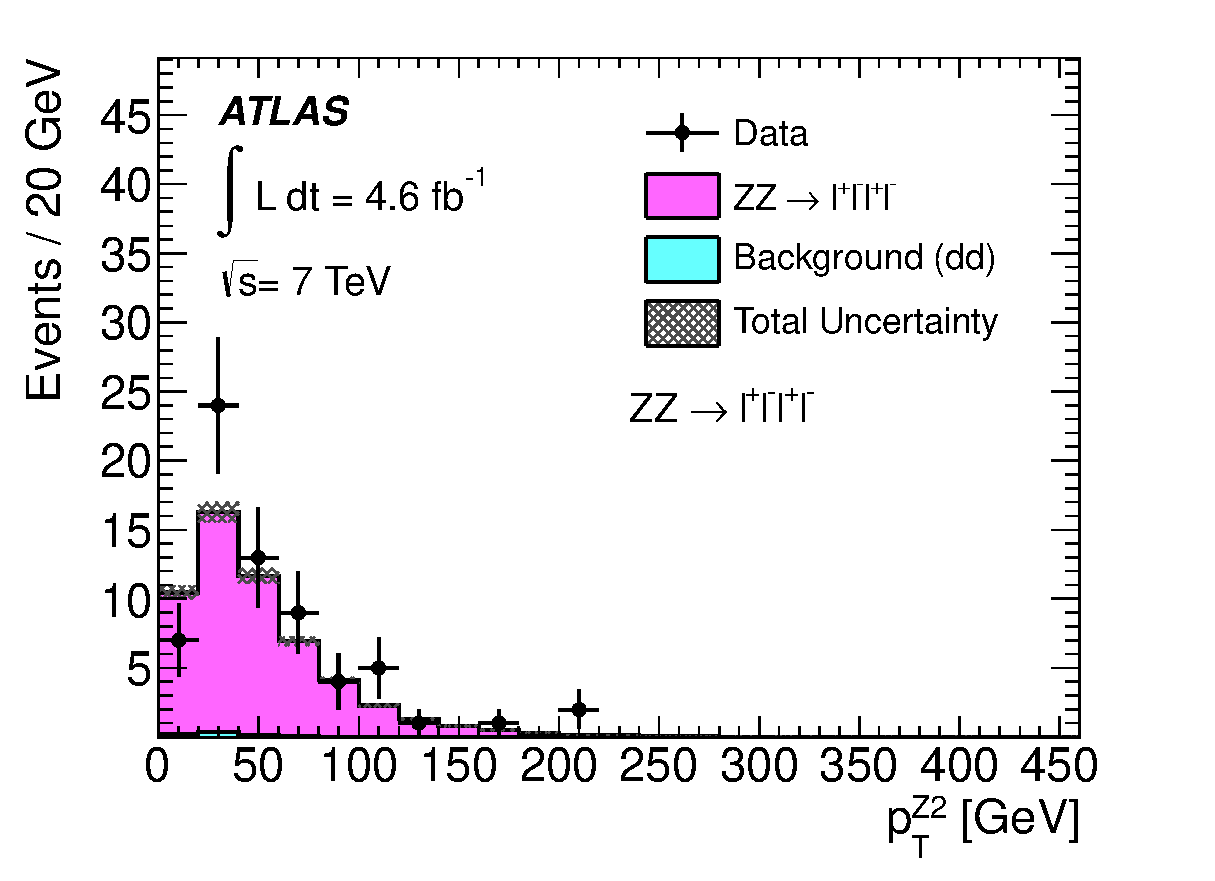
\includegraphics[width=0.47\textwidth]{7TeV/h_4l_ZZ_Z2_pt}
     }
    \caption[Kinematic distributions for events passing the \ZZ\ selection in
    the 7~\tev\ data.]
    {Kinematic distributions for events passing the \ZZ\ selection in
    the 7~\tev\ data: (a) transverse momentum $\pT^{\ZZ}$ and (b) invariant mass $m^{\ZZ}$ of the 
    four-lepton system, (c) transverse momentum of the leading
    \dilep\ pair $\pt^{Z1}$, and (d) transverse momentum of the subleading
    \dilep\ pair $\pt^{Z2}$. The points represent the observed data and the 
    histograms show the prediction from simulation, where the background
    is normalized to the data-driven (dd) estimate as described in
    ~\chap{BackgroundEstimate}. The shaded band 
    shows the combined statistical and systematic uncertainty on the prediction. 
    }
    \label{fig:zzdists-ZZ-seven}
    \end{center}
\end{figure}

% 7 TeV, ZZ*, ZZ_pt / ZZ_m
\begin{figure}[htbp]
\begin{center}
    \subfigure[]{
    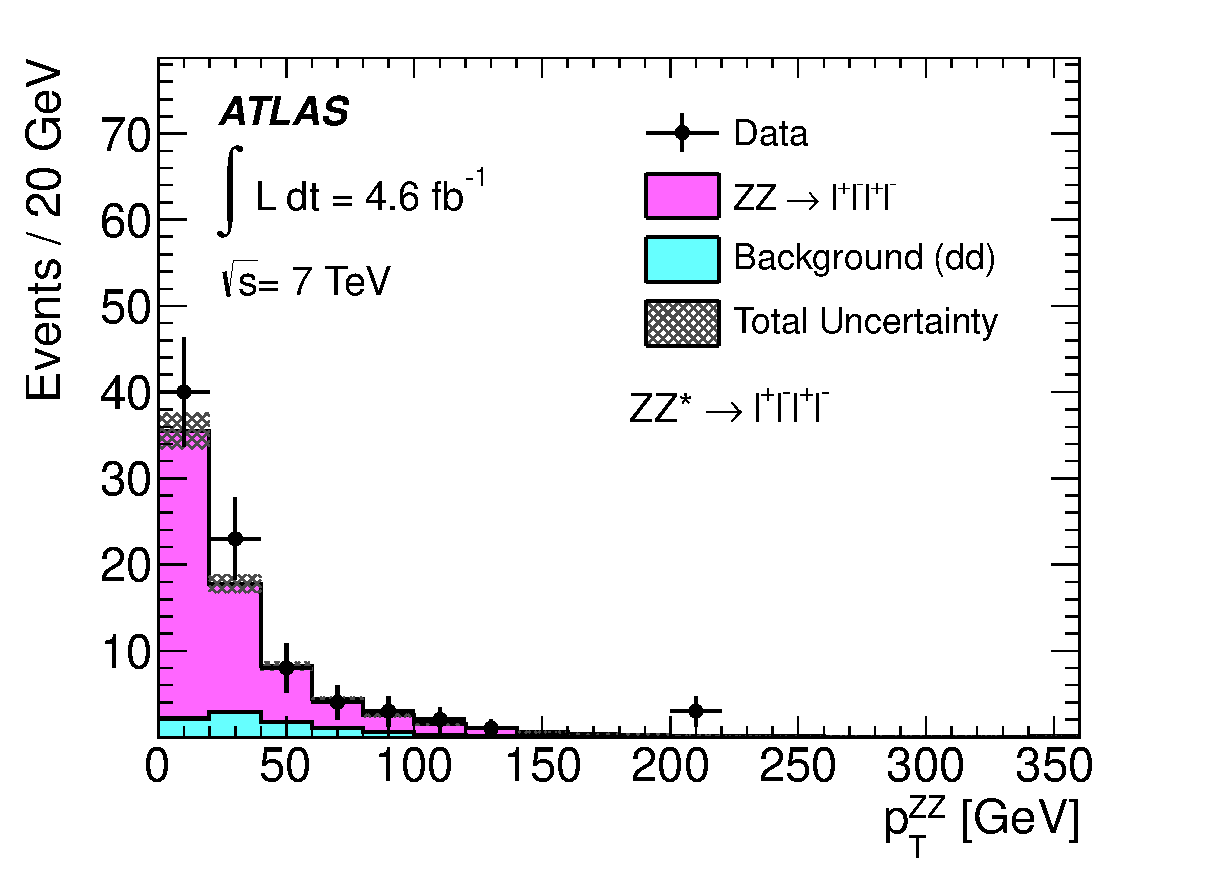
\includegraphics[width=0.47\textwidth]{7TeV/h_4l_ZZs_ZZ_pt}
    }
    \subfigure[]{
    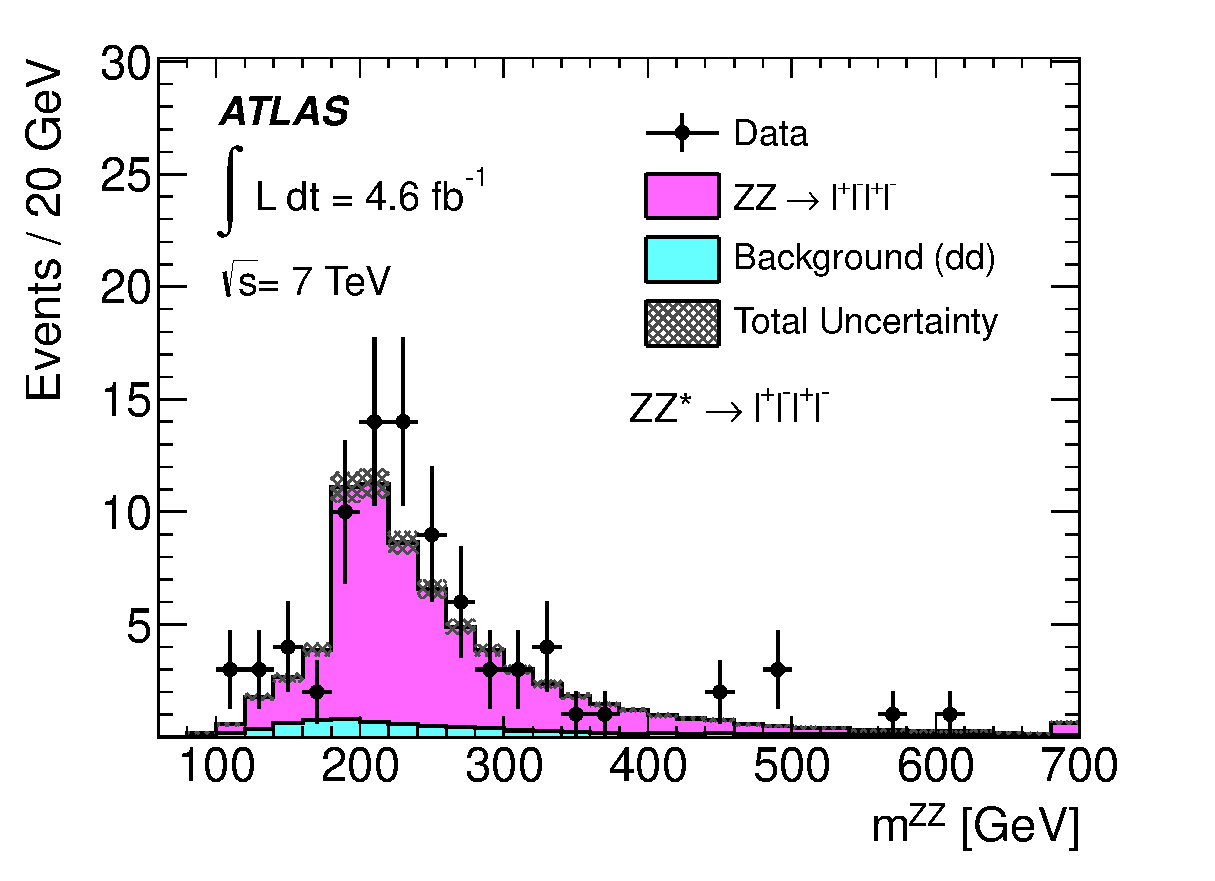
\includegraphics[width=0.47\textwidth]{7TeV/h_4l_ZZs_ZZ_m}
    }
    \subfigure[]{
    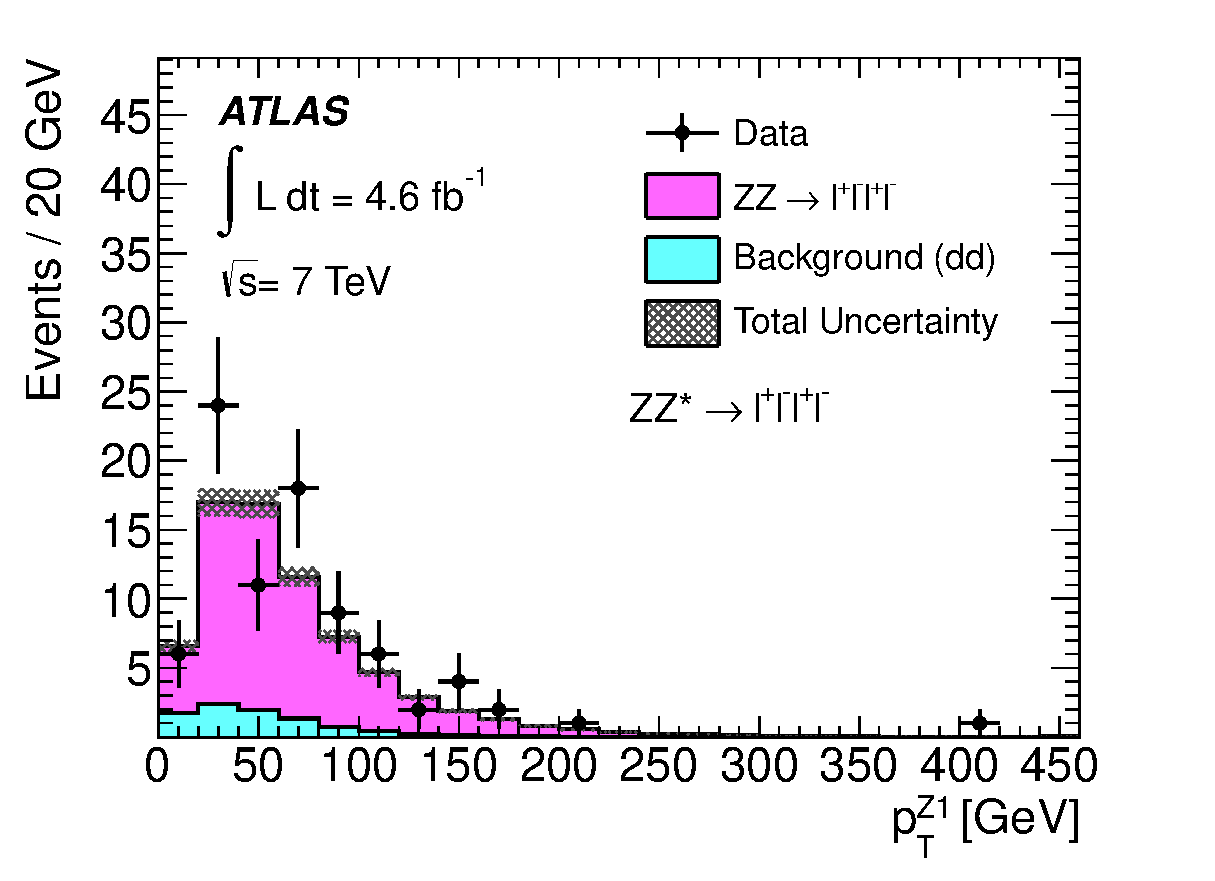
\includegraphics[width=0.47\textwidth]{7TeV/h_4l_ZZs_Z1_pt}
    }
    \subfigure[]{
    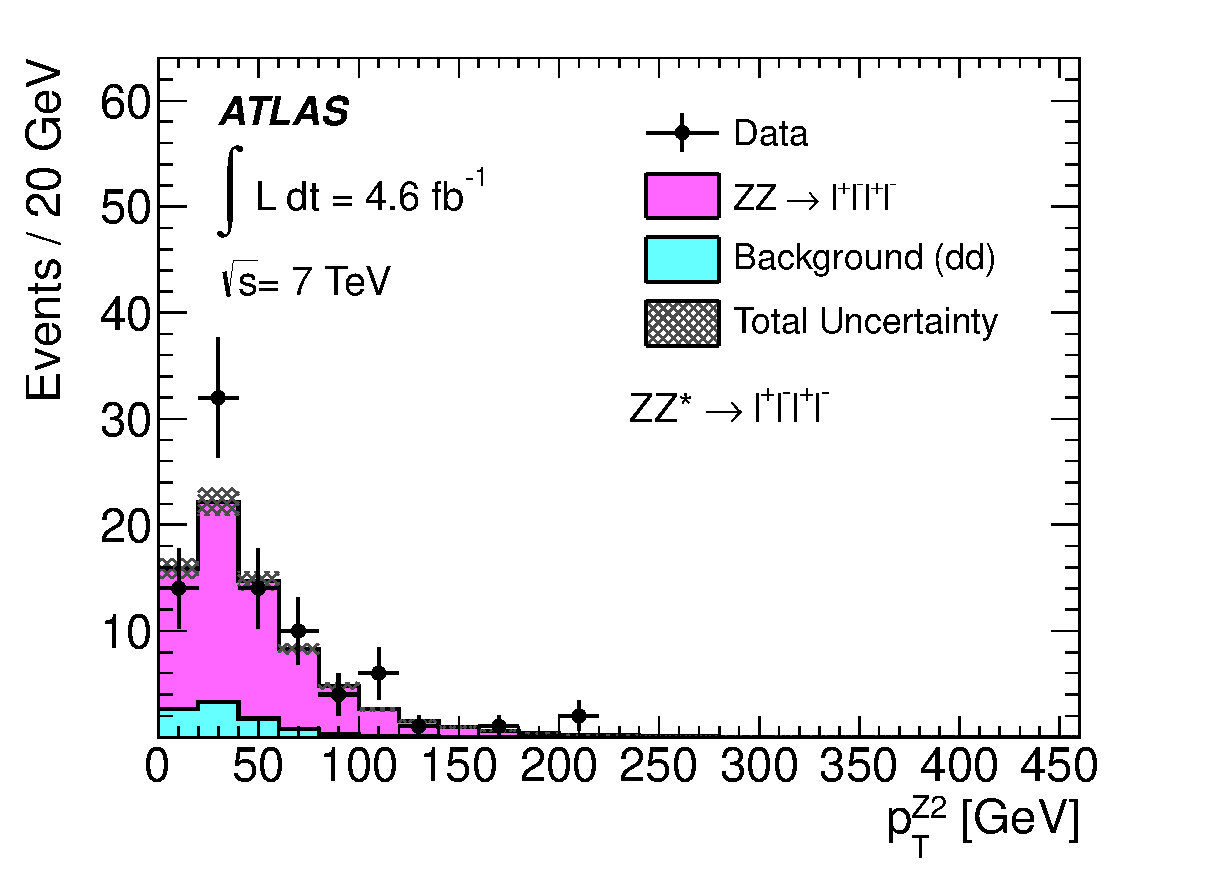
\includegraphics[width=0.47\textwidth]{7TeV/h_4l_ZZs_Z2_pt}
    }
    \caption[Kinematic distributions for events passing the \ZZs\ selection in
    the 7~\tev\ data.]
    {Kinematic distributions for events passing the \ZZs\ selection in
    the 7~\tev\ data: (a) transverse momentum $\pT^{\ZZ}$ and (b) invariant mass $m^{\ZZ}$ of the 
    four-lepton system, (c) transverse momentum of the leading
    \dilep\ pair $\pt^{Z1}$, and (d) transverse momentum of the subleading
    \dilep\ pair $\pt^{Z2}$. The points represent the observed data and the 
    histograms show the prediction from simulation, where the background
    is normalized to the data-driven (dd) estimate as described in
    ~\chap{BackgroundEstimate}. The shaded band 
    shows the combined statistical and systematic uncertainty on the prediction. 
    }
\end{center}
    \label{fig:zzdists-ZZs-seven}
\end{figure}

\section{Cross Section Measurement}

As discussed in~\sec{}, the \cx\ is first measured in a fiducial phase-space
corresponding to the experimental selections (the \intro{fiducial \cx}), in
order to reduce systematic uncertainties associated with the extrapolation. The
fiducial \cx\ is then extrapolated to the total \ZZ\ \cx. The definition of the
fiducial phase-space was given in~\sec{}, and is slightly different for the
7~\tev\ and 8~\tev\ analyses due to the differing experimental selections.

\subsection{Fiducial Cross Section}

For a given \ZZllll\ final state the fiducial cross section is defined as:

\begin{equation}\label{eq:xsecfid_fourl}
\sigmaFid = \frac{\NObs - \NBg}{\mathcal{L} \times \CZZ^{\lllplp}}
\end{equation}
where \NObs\ and \NBg\ are the number of observed and
background events respectively, $\mathcal{L}$ is the integrated luminosity and
$\CZZ^{\lllplp}$ is the reconstruction acceptance factor for the \lllplp\
final-state, as defined in~\sec{objSel-CZZ}.

The \cx\ is estimated using a maximum profile likelihood technique, by
maximising the \intro{profile likelihood function, \L} with respect to the \cx.
\L is the product of the Poisson probability distribution ($P$) to observed $N$ events given a
\cx $\sigma$, reconstruction acceptance \CZZ\ and background $b$ and Gaussian
distributions to describe the nuisance parameters due to uncertainties on \CZZ\
and on $b$:

\begin{equation}
   \L(\sigma, \CZZ', b'; \Delta_{b}, \Delta_{C_{ZZ}}, N) = P(\sigma, \CZZ^\prime,
   b^\prime; N)\times G(\CZZ^\prime; C_{ZZ}, \Delta_{C_{ZZ}}) \times G(b^\prime; b, \Delta_{b}).
\end{equation}

The Poisson probability function to observe $N$ events given and expected
number of signal events $s$ and expected background $b$ is:

\begin{equation}
P(\sigma, C_{ZZ}, b; N) =
\frac{e^{-(s(\sigmaFid, \CZZ)+b)}\cdot
     \left(s(\sigmaFid, \CZZ)+b\right)^{N}}
     {N!},
\end{equation}
where :

\begin{equation}
   s(\sigmaFid, \CZZ) = \sigma^\mathrm{fid}\times\mathcal{L}\times\CZZ \\
\end{equation}

In practice, for computational convenience $-\ln(L)$ is minimised rather
than maximising $L$, however the procedures are equivalent.

\subsection{Total Cross Section}
The total cross-section is defined as:

\begin{equation}\label{eq:xsectot_fourl}
\sigmaTot = \frac{ \NObs - \NBg}{\mathcal{L} \times
BR\{\zzllll\} \times \AZZ \times \CZZ^{\lllplp}}
\end{equation}
where \AZZ\ is the \intro{fiducial acceptance factor}, which is equal to the
fraction of \ZZ\ events which fall into the fiducial phase-space:

\begin{equation}
\AZZ = \frac{ N^{\rm MC\ Fiducial Volume}_{{\rm Generated}\ ZZ} }{ N^{{\rm MC\
All}}_{{\rm Generated}\ ZZ} }
\end{equation}

%The $ZZ\rightarrow\tau\tau\nu\nu$ with subsequent $\tau\tau\rightarrow
%\ell\ell$ contamination to the direct decay of $\zzllvv$
%is negligible.  This is due to the tight $Z$ mass
%requirement of $76<M_{ll}<106\,\mathrm{GeV}$ in the fiducial volume.  
%Less than $0.1$\% of $\zzllvv$ are found in the 
%signal region. The contribution of  $ZZ\rightarrow\tau\tau\ell\ell$ decays to
%selected events in the \zzllll\ decay channel is 0.2\% for the \ZZ\ selection, and
%1.8\% for the \ZZs\ selection; the higher value being a result of the looser mass
%cut (see Table~\ref{table:CZZcontaminations}).

%The combination of these cross sections could use a basic approach
%where one uses the total sum over channels of observed events, total
%sum over channels of expected background events, and weighted sum over
%channels of acceptances.  This method would give highest weight in the
%combination to the highest statistics channel and would not
%necessarily take into account better signal-to-background ratios in
%other channels.  One could also use a minimum $\chi^{2}$ approach,
%which amounts to a covariance weighted average.  Unfortunately this
%combination needs higher statistics than we currently have.
%
%We use a maximum log-likelihood approach to calculate the combined
%cross section.  This approach takes into account the Poisson
%statistics of our samples as well as the systematic uncertainties.
%This is described in the next section~\ref{sec:CrossSecCalc}.
%
%We estimate the cross section by maximizing the profile likelihood function
%$L$ with respect to the cross section $\sigma$.  We
%merge the two channels before maximizing $L$.
%
%The profile likelihood function for the fiducial cross section is the product of a Poisson probability
%distribution ($P$) and Gaussian distribution function ($G$) for the  nuisance parameters. The likelihood 
%function includes parameters from the two decay channels: channel 1 (\zzlmlplmlp) and channel 2 (\zzllvv). 
%$C_{1}$ and $C_{2}$ represent $C_{ZZ}$ for each channel; the $C_{1,2}'$ terms are allowed to float with a 
%Gaussian constraint, and the $C_{1,2}$ terms are the mean values calculated from Monte Carlo. The uncertainties in $C_{1,2}$ are split into 
%two groups: those uncertainties which are uncorrelated between channels and those which are correlated.  
%The variables $\overrightarrow{\beta}=(\beta_{1},...,\beta_{k})$ represent the variations in the correlated uncertainties 
%($\overrightarrow{\Delta{C_{1}}}^{\rm corr}=(\Delta{C_{1;i=1}}^{\rm corr},...,\Delta{C_{1;i=k}}^{\rm corr}$ and 
%$\overrightarrow{\Delta{C_{2}}}^{\rm corr}=(\Delta{C_{2;i=1}}^{\rm corr},...,\Delta{C_{2;i=k}}^{\rm corr}$)
%and are distributed according to a single Gaussian distribution 
%function with $\sigma=1$ and $\mu=0$ ($\alpha$ for $A_{ZZ}$ uncertainties). The electron uncertainties, muon  
%uncertainties, trigger uncertainties, and PDF uncertainties are treated as 100\% correlated between the \zzllvv\ and \zzlmlplmlp\ channels.
%We also calculated the total cross section assuming that the uncertainties are uncorrelated between the two channels, and found that our 
%correlation assumption is more conservative.
%The background uncertainties are treated as totally uncorrelated across the two channels. 
%For $k$ correlated uncertainties, the likelihood is written as follows:
%\begin{eqnarray} \nonumber
%&L( (\sigma^{\rm total}\ {\rm or}\ \sigma^{\rm fid}_{1}, \sigma^{\rm fid}_{2}), \overrightarrow{\beta}, b_{1}', b_{2}';
% C_{1}, C_{2}, \Delta{b}_{1}, \Delta{b}_{2}, \Delta{C_{1}^{\rm uncorr}}, \Delta{C_{2}^{\rm uncorr}}, 
%\overrightarrow{\Delta{C_{1}}}^{\rm corr}, \overrightarrow{\Delta{C_{2}}}^{\rm corr}, N) =& \\ \nonumber
%%
%& P((\sigma^{\rm total}\ {\rm or}\ \sigma^{\rm fid}_{1}), \overrightarrow{\beta}, b_{1}'; C_{1}, \Delta{C_{1}}^{\rm uncorr}, \overrightarrow{\Delta{C_{1}}}^{\rm corr}, N) \cdot 
%P((\sigma^{\rm total}\ {\rm or}\ \sigma^{\rm fid}_{2}), \overrightarrow{\beta}, b_{2}'; C_{2}, \Delta{C_{2}}^{\rm uncorr}, \overrightarrow{\Delta{C_{2}}}^{\rm corr}, N) \cdot& \\ 
%%
%&\Gamma(\overrightarrow{\beta},b_{1}',b_{2}';b_{1},b_{2},\Delta{b_{1}},\Delta{b_{2}}).& \nonumber
%\end{eqnarray}
%
%Where the $\Gamma$ function contains all of the Gaussian constraints:
%
%\begin{equation}
%\prod_{i=1}^{i\leq{k}} G(\beta_{i}; 0, 1) \cdot G(\beta_{1}^{\rm uncorr}; 0, 1) \cdot
%G(\beta_{2}^{\rm uncorr}; 0, 1) \cdot 
%G(b_{1}'; b_{1}, \Delta{b_{1}}) \cdot G(b_{1}'; b_{1}, \Delta{b_{1}}).
%\end{equation}
%
%For the total cross section, we append $G(A_{ZZ}^\prime; A_{ZZ}, \Delta_{A_{ZZ}})$ to the likelihood to account for the uncertainty on
%the fiducial acceptance $A_{ZZ}$.
%
%The Poisson function for the number
%of observed events $N$ is
%\begin{equation}
%P(\sigma, C_{ZZ}, b; N) =
%\frac{e^{-(s(\sigma, C_{ZZ})+b)}\cdot
%     \left(s(\sigma, C_{ZZ})+b\right)^{N}}
%     {N!},
%\end{equation}
%where the number of signal events is a function of the cross section
%and other quantities such as the integrated luminosity and correction
%factors. We note
%aside that $-\ln(L)$ is minimized for computational convenience rather
%than maximizing $L$.
%
%For the fiducial and the total cross sections, the number of signal events is
%%($\sigma = \sigma_\mathrm{fid} \textrm{ and } \sigma_\mathrm{tot}$,%respectively) 
%\begin{eqnarray}
%& s(\sigma_\mathrm{fiducial}, C_{1}) = \sigma_\mathrm{fiducial}\cdot\mathcal{L}\cdot(C_{1}+\beta^{\rm uncorr}\Delta{C_{1}^{\rm uncorr}}+\overrightarrow{\beta}\cdot\overrightarrow{\Delta{C_{1}^{\rm corr}}}) & \\
%& s(\sigma_\mathrm{total}, C_{1}) = \mathrm{BR_1} \cdot \sigma_\mathrm{total}\cdot\mathcal{L}\cdot & \\ \nonumber
%&(C_{1}+\beta^{\rm uncorr}\Delta{C_{1}^{\rm uncorr}}+\overrightarrow{\beta}\cdot\overrightarrow{\Delta{C_{1}^{\rm corr}}})
%\cdot(A_{1}+\alpha^{\rm uncorr}\Delta{A_{1}^{\rm uncorr}}+\overrightarrow{\alpha}\cdot\overrightarrow{\Delta{A_{1}^{\rm corr}}})& ,
%\end{eqnarray}
%%where the factor of 4 accounts for the lepton combinatorics of $\zzllvv$. 
%The $A_{ZZ}$ in the latter formula accounts for the fiducial volume of the measurement. 
%
%Two types of uncertainties, statistical and systematic, are associated
%with the cross section measurement.  
%Table~\ref{ta:CrossSection} summarizes the fiducial and total cross section results. 
%
%\renewcommand{\arraystretch}{1.7}
%\begin{table}[htbp]
% \centering
% \begin{tabular}{|cc|c|}
%   \hline
%\multirow{3}{*}{\zzllll\ Fiducial} & $\zzllll$ & $\zzllllfid$ \\
%                          & $\zzeeee$ & $\zzeeeefid$ \\
%                          & $\zzeemm$ & $\zzeemmfid$ \\
%                          & $\zzmmmm$ & $\zzmmmmfid$ \\ 
%                          & $\ZZs\ra\ell\ell\ell'\ell'$ & $\zzsllllfid$ \\
%\hline
%\multirow{3}{*}{\zzllvv\ Fiducial} & $\zzllvv$ & $\zzllvvfid$ \\
%                          & $\zzeevv$ & $\zzeevvfid$ \\ 
%                          & $\zzmmvv$ & $\zzmmvvfid$ \\ 
%\hline
% \multirow{3}{*}{Total}   & $ZZ$ (combined) & $\zztot$ \\
%                          & $\zzllll$ & $\zzlllltot$ \\
%                          & $\zzllvv$ & $\zzllvvtot$ \\
%\hline
%\end{tabular}
%\caption{\label{ta:CrossSection}Results}
%\end{table}
